\documentclass[a4paper,10pt]{scrartcl}
\usepackage[utf8]{inputenc}
\usepackage[ngerman]{babel}
\usepackage{ngerman}
\usepackage[T1]{fontenc}
\usepackage{setspace}
\usepackage{graphicx}
\usepackage{multirow, multicol}
\usepackage{pdflscape}
\usepackage{epstopdf}
\usepackage{tabularx}
\usepackage{amsmath,amsfonts,amssymb}
\usepackage{natbib}
\usepackage{textcomp}
\usepackage{bm}
\usepackage{titlesec}
\usepackage[parfill]{parskip}
\usepackage{color}
\definecolor{black}{rgb}{0,0,0}
\usepackage[colorlinks=true, breaklinks=true, linkcolor=black, menucolor=black, urlcolor=black, citecolor=black, anchorcolor=black, filecolor=black, menucolor=black]{hyperref}
\usepackage[paper=a4paper,left=30mm,right=30mm,top=30mm,bottom=30mm]{geometry} 
\setcounter{tocdepth}{10}\setcounter{secnumdepth}{10}\setlength{\columnsep}{2em}
\titleformat{\paragraph}[hang]{\sffamily\bfseries}{\theparagraph}{.5em}{}
\titleformat{\subparagraph}[hang]{\sffamily\bfseries}{\thesubparagraph}{.5em}{}
\deffootnote{1em}{1em}{\textsuperscript{\thefootnotemark\ }}
\begin{document}
\title{Subversion}
\author{von Stefan Arndt, Christian Autermann und Dustin Demuth}
\date{\today}
\maketitle
\tableofcontents
\newpage
\onehalfspacing
\section{Versionierung}%%% dustin

\subsection{Zweck von Versionierung}

Versionierung - eigentlich Versionsverwaltung - beschäftigt sich mit der Erfassung von Änderungen an Dokumenten. Hierfür werden, in dem zu verwaltendem Archiv, für jede Datei Zeitstempel und Nutzerdaten erfasst, welche zu jedem Zeitpunkt wiederhergestellt werden können. Somit wird eine lückenlose Nachvollziehbarkeit von Textänderungen gewährleistet. Versionsverwaltung ist somit eine Art des Variantenmanagements, welches hauptsächlich in der Industrie eingesetzt wird. Dieses Konzept hat sich auf die Softwareentwicklung durchgesetzt. 

\subsection{Geschichtliches}
SVN entstand als Ersatz für CVS (Content Versioning System). Jedoch hatte CVS immense Einschränkungen, da es nach den Orten der Änderungen Versionierte und nicht nach der zeitlichen Abfolge. Das brachte die SVN-Entwickler dazu "`Schönheitsreperaturen"' an CVS durchzuführen. Dies begann im Februar 2000. Daraufhin verbreitete sich Subversion selbst, nachdem die Entwickler von CVS auf SVN umstellten. Die erste stabile Version erschien im Jahr 2004.

\subsection{Aufbau der Versionierung}
In der Architektur von Subversion wurde das alte Schema P: L-T (Projectarchive: Location-Time) von CVS zu P: T-L umgewandelt. Dies schaffte den Vorteil, dass SVN anschaulicher wurde und somit die Erfahrungsgemäße Realität an Änderungen besser nachstellen konnte. Hierbei bezieht sich das Versionsschema nicht mehr auf einzelne Dateien - wie in CVS - sondern auf das ganze Projekt. Somit lässt sich einfacher eine Konkrete Version beschreiben. \\
\section{Wichtige Begriffe}
\subsection{Repository}
Unter einem Repository versteht man ein zentrales, auf einem Server lagerndes Archiv, das über die gesamte Versionsgeschichte jeder Datei, die im Repository abgelegt wurde, verfügt.\\
Da man in der Regel für jedes Projekt ein eigenes Repository benutzt, ist ein Subversion-Server in der Lage mehrere Repositories zu verwalten.\\
Zum Bearbeiten der versionierten Dateien lädt man sich eine lokale Arbeitskopie aus dem Repository und lädt anschließend die veränderten Dateien in das Repository.
\subsection{Revision}
Im jedem Repository gibt es die sogenannte Revisionsnummer. Beim Anlegen eines Repositories beträgt sie null und wird bei jeder eingereichten Änderung um 1 inkrementiert. Für jede versionierte Datei wird zusätzlich die Revisionsnummer der letzten Bearbeitung gespeichert.\\
Durch Angabe einer Nummer lässt sich die Version einer Datei eindeutig bestimmen und so auch der Zustand einer Datei oder des gesamten Projektes zu einem bestimmten Zeitpunkt wiederherstellen.\\
Die aktuellste des Repository nennt man auch \emph{head} und die lokale, noch nicht eingereichte Revision, heißt \emph{base}.
\subsection{Verzeichnisstruktur}
Unabhängig von der Art des Projektes hat sich eine Verzeichnisstruktur etabliert, die mehrere Entwicklungsstränge ermöglicht.\\
Der Hauptentwicklungszweig lagert in \emph{trunk}, Nebenzweige werden in \emph{branch} abgelegt und \emph{tag} enthält benannte Versionen.\\
Da in Subversion beim kopieren einer Datei, nicht die Datei kopiert wird, sondern nur ein neuer Verweis in der Datenbank angelegt wird, ist es möglich ohne zusätzlichen Speicherbedarf Dateien zu kopieren und deren Versionsgeschichte zu erhalten. Möchte man nun eine eine benannte Version (bspw. ein Release Candidate o.ä.) erstellen, reicht es mit Hilfe von Subversion das Projekt aus \emph{trunk} nach \emph{tag} zu kopieren und dort umzubennen. Subversion legt dabei nur eine Verknüpfung unter dem neuen Namen mit der Versionsgeschichte der Originaldateien an.\\
Gleiches geschieht beim Erstellen eines neuen Entwicklungszweiges in \emph{branch}.
\section{Konflikte}
\begin{figure}[!htb]
\centering
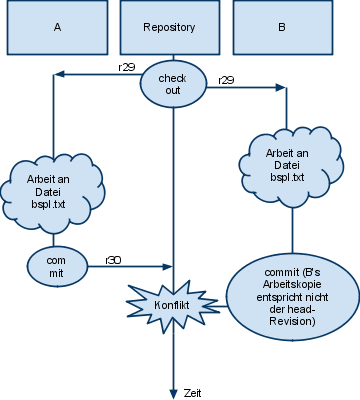
\includegraphics[width=0.7\textwidth]{konflikt}
\caption{Konflikt beim gleichzeitigen Bearbeiten einer Datei (Quelle: eigene Darstellung).}
\label{fig:konflikt}
\end{figure}
Subversion erlaubt das gleichzeitige Arbeiten mehrerer Personen an der selben Datei. Dies führt zwangsläufig zu Konflikten wie Abbildung \ref{fig:konflikt} zeigt. Subversion bietet hierfür zwei Lösungen an.
\subsection{Merge}
In Abbildung \ref{fig:konflikt} kann B nicht einfach seine Änderungen commiten, da dies alle Änderungen, die A gemacht hat, verwerfen würde. Daher ist B gezwungen die im Konflikt stehenden Dateiversionen zu verschmelzen (zu mergen). Dies kann automatisch (bsplw. wenn sich die Veränderungen nich gegenseitig beeinflussen) oder von Hand geschehen. Um dies zu Vereinfachen gibt es eine Vielzahl Tools die einen synoptischen Vergleich der Dateien ermöglichen und die Unterschiede visualisieren.

\subsection{Locks}
Locks eigenen sich besonders für binäre Dateien, bei denen ein synoptischer Vergleich der beiden in Konflikt stehenden Dateien nicht möglich ist.\\
Um Konflikte zu Verhindern wird bevor die Datei bearbeitet wird eine Sperre (der sogenannte Lock) für die Datei angefordert. Alle anderen Personen können ab diesem Zeitpunkt zwar die Datei lesen und bearbeiten, allerdings nicht commiten. Erst mit dem nächsten Commit des Lock-Inhabers wird die Datei wieder für andere freigegeben.\\
Da man eine von jemand Anders gesperrte Datei in seiner Arbeitskopie beliebig verändern kann und über ein Lock nur bei einem versuchten Commit informiert wird, empfiehlt es sich vor jedem Bearbeiten den Status einer Binärdatei zu überprüfen um unnötige Arbeit zu verhindern.

\section{Die Kommandozeile}

\section{Graphical Frontends}
Es gibt eine große Auswahl von graphischen Benutzeroberflächen um auf Subversion-Repositorys zuzugreifen. Sie vereinfachen den Umgang mit SVN enorm, da komplett auf die Kommandozeilen Eingabe verzichtet wird.\\
Drei verschiedene Arten von GUIs werden wir hier nun kurz  vorstellen:
\subsection{SmartSVN}
SmartSVN ist ein eigenständies Programm, das auf den Betriebssystemen Linux, UNIX, Mac OS X, Windows lauffähig ist. Im Internet ist eine gratis Demoversion für 30 Tage auffindbar, wenn man allerdings die Vollversion benutzen möchte, muss man dafür zahlen.\\
Neben dem Standalone-Client integriert sich SmartSVN unter Windows zusätzlich auch noch in den Explorer (Abbildung \ref{fig:smart1}). Das Menü bietet eine übersichtliche Dateiverwaltung (Abbildung \ref{fig:smart2}) und optisch gut aufbereitete Vergleiche der Versionen an (Abbildung \ref{fig:smart3}).
Neben dem HTTP-Protokoll, werden auch noch HTTPS, SVN, und SVN+SSH unterstützt\footnote{Quelle: \url{http://www.syntevo.com/smartsvn}}.
\begin{figure}[!htb]
        \centering
        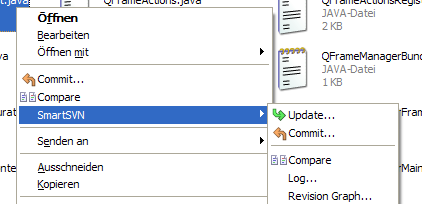
\includegraphics[width=.8\textwidth]{1_smartsvn1.png}
        \caption{SmartSVN: Shell-Integration}
        \label{fig:smart1}
\end{figure}
\begin{figure}[!htb]
        \centering
        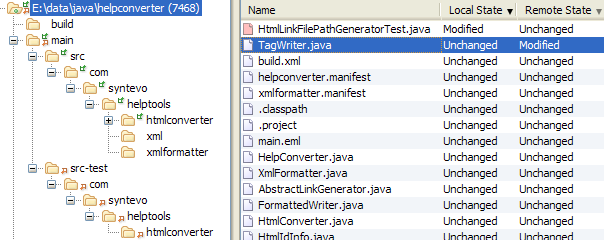
\includegraphics[width=.9\textwidth]{2_smartsvn2.png}
        \caption{SmartSVN: Dateiverwaltung}
        \label{fig:smart2}
\end{figure}
\begin{figure}[!htb]
        \centering
        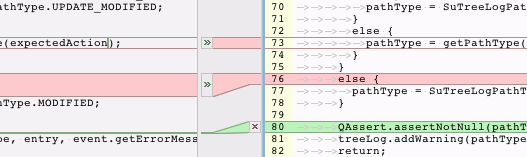
\includegraphics[width=.9\textwidth]{3_smartsvn3.png}
        \caption{SmartSVN: Unterschiedskontrolle}
        \label{fig:smart3}
\end{figure}
\subsection{Tortoise SVN}
Tortoise hingegen ist ein kostenloser Windows-Client der unter der GNU GPL Lizenz steht. Es integriert sich ebenfalls in den Windows-Explorer und ist deshalb ebenfalls außerhalb und unabhängig von einer IDE verwendbar. Im Gegensatz zu SmartSVN ist TortoiseSVN aber kein standalone-Client, sondern bietet nur die reine Shell-Extension (Abbildung \ref{fig:tortoise1}).
Zur Zeit ist die Software in 34 Sprachen verfügbar und es werden standardmäßig die Protokolle http, https, svn, svn+ssh, file und svn+xxx unterstützt\footnote{Quelle: \url{http://tortoisesvn.tigris.org/}, \url{http://de.wikipedia.org/wiki/TortoiseSVN}}.
\begin{figure}[!htb]
	\centering
	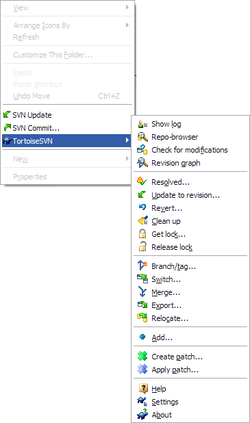
\includegraphics[width=.45\textwidth]{4_turtoise1.png}
	\caption{Bildbeschreibung}
	\label{fig:tortoise1}
\end{figure}  
\subsection{Subclipse SVN}
Subclipse ist die dritte GUI Variante, die nun hier vorgestellt wird. Anders als die beiden vorhergegangenen Programme integriert sich Subclipse direkt in die Entwicklungsumgebung Eclipse.\\
Das Eclipse-Plugin steht unter der EPL-Lizenz und ist unter den Betriebssystemen Linux, Mac OS X und Windows lauffähig. Subclipse unterstützt die folgenden Protokolle: http, https, svn, svn+ssh und file. Neben dem Vorteil die Dateien direkt vom SVN Repository in die IDE (siehe Abbildung \ref{fig:subclipse1}) zu laden, bietet Subclipse zusätzlich ansprechende Features wie z.B. die Generierung von Versionsgraphen.\footnote{Quelle: \url{http://subclipse.tigris.org/}}
\begin{figure}[!htb]
        \centering
        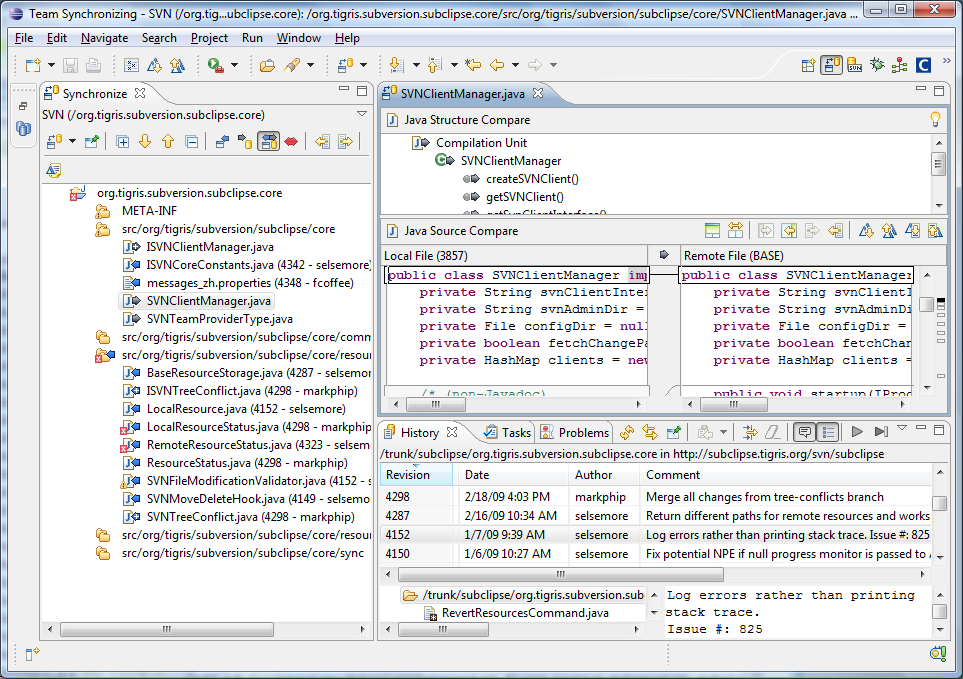
\includegraphics[width=1\textwidth]{5_subclipse1.png}
        \caption{Subclipse: Eclipse Synchronize View}
        \label{fig:subclipse1}
\end{figure}

\end{document}  
